%----------------------------------------------------------------------------------------
%	PACKAGES AND OTHER DOCUMENT CONFIGURATIONS
%----------------------------------------------------------------------------------------

\documentclass[twoside]{article}

\usepackage{lipsum} % Package to generate dummy text throughout this template
\usepackage{algorithm}
\usepackage{algpseudocode}
\usepackage[sc]{mathpazo} % Use the Palatino font
\usepackage[T1]{fontenc} % Use 8-bit encoding that has 256 glyphs
\linespread{1.05} % Line spacing - Palatino needs more space between lines
\usepackage{microtype} % Slightly tweak font spacing for aesthetics

\usepackage[hmarginratio=1:1,top=32mm,columnsep=20pt]{geometry} % Document margins
\usepackage{multicol} % Used for the two-column layout of the document
% Custom captions under/above floats in tables or figures
\usepackage[hang, small,labelfont=bf,up,textfont=it,up]{caption}
\usepackage{booktabs} % Horizontal rules in tables
\usepackage{float}
\usepackage{hyperref} % For hyperlinks in the PDF

\usepackage{lettrine}
\usepackage{paralist}

\usepackage{abstract} % Allows abstract customization
\renewcommand{\abstractnamefont}{\normalfont\bfseries} % Set the "Abstract" text to bold
\renewcommand{\abstracttextfont}{\normalfont\small\itshape} % Set the abstract itself to small italic text

\usepackage{titlesec} % Allows customization of titles
\renewcommand\thesection{\Roman{section}} % Roman numerals for the sections
\renewcommand\thesubsection{\Roman{subsection}} % Roman numerals for subsections
\titleformat{\section}[block]{\large\scshape\centering}{\thesection.}{1em}{}
\titleformat{\subsection}[block]{\large}{\thesubsection.}{1em}{}

\usepackage{fancyhdr} % Headers and footers
\pagestyle{fancy} % All pages have headers and footers
\fancyhead{} % Blank out the default header
\fancyfoot{} % Blank out the default footer
\fancyhead[C]{ESE650 Learning in Robotics $\bullet$ May 2014 $\bullet$ Project 6}
\fancyfoot[RO,LE]{\thepage} % Custom footer text

\usepackage[pdftex]{graphicx}
\usepackage{epstopdf}
\usepackage{subfigure}
\usepackage{amsmath,amssymb,amsopn,amstext,amsfonts}
\usepackage{url}
\usepackage[usenames,dvipsnames]{color}
\usepackage{siunitx}
\usepackage{amsmath}
\usepackage{amsfonts}
\usepackage{amssymb}

\graphicspath{{fig/}}
\newcommand{\x}{\mathbf{x}}
\newcommand{\z}{\mathbf{z}}
\newcommand{\e}{\mathbf{e}}
\newcommand{\F}{\mathbf{F}}
\newcommand{\J}{\mathbf{J}}
\newcommand{\omg}{\mathbf{\Omega}}
\newcommand{\W}{\mathcal{W}}
\newcommand{\X}{\mathcal{X}}
\newcommand{\Y}{\mathcal{Y}}
\newcommand{\Z}{\mathcal{Z}}
\newcommand{\red}[1]{\textcolor{red}{#1}}
\newcommand{\brown}[1]{\textcolor{brown}{#1}}

%-------------------------------------------------------------------------------
%	TITLE SECTION
%-------------------------------------------------------------------------------

\title{\vspace{-15mm}\fontsize{24pt}{10pt}\selectfont\textbf{Multi-robot Pose Graph Optimization}} % Article title

\author{
\large
\textsc{Chao Qu}\thanks{A thank you or further information}\\[2mm] % Your name
\normalsize University of Pennsylvania \\ % Your institution
\normalsize \href{mailto:quchao@seas.upenn.edu}{quchao@seas.upenn.edu} % Your email address
\vspace{-5mm}
}
\date{}

%-------------------------------------------------------------------------------

\usepackage{graphicx}
\begin{document}


\maketitle % Insert title

\thispagestyle{fancy} % All pages have headers and footers

%-------------------------------------------------------------------------------
%	ABSTRACT
%-------------------------------------------------------------------------------

%\begin{abstract}
%
%\noindent Hey, I'm just an abstract. % Dummy abstract text
%
%\end{abstract}

%-------------------------------------------------------------------------------
%	ARTICLE CONTENTS
%-------------------------------------------------------------------------------

%-------------------------------------------------------------------------------
%	INTRODUCTION
%-------------------------------------------------------------------------------

\begin{multicols}{2} % Two-column layout throughout the main article text

\section{Introduction}
\lettrine[nindent=0em,lines=2]{S}LAM is recently a hot topic in robotics research field. SLAM stands for Simultaneous Localization and Mapping. The goal of SLAM is to enable the robot with the ability to build a map of an unknown environment while simultaneously localize itself and navigate around. One line of SLAM research is to form a graph whose nodes are the poses of the robot in time and edges are spatial constraints between the poses. The edges can be obtained from robot odometry or observation of the environment. Once such a graph is constructed, it can be solved using conventional non-linear optimization techniques. In this project, our goal is to apply this SLAM methods to multiple robots and find the best spatial configuration of all robot poses that is mostly consistent with 2D laser scan measurements. A raw trajectory of all robots is shown in Fig. \ref{fig:raw_traj}.

\begin{figure}[H]
\centering
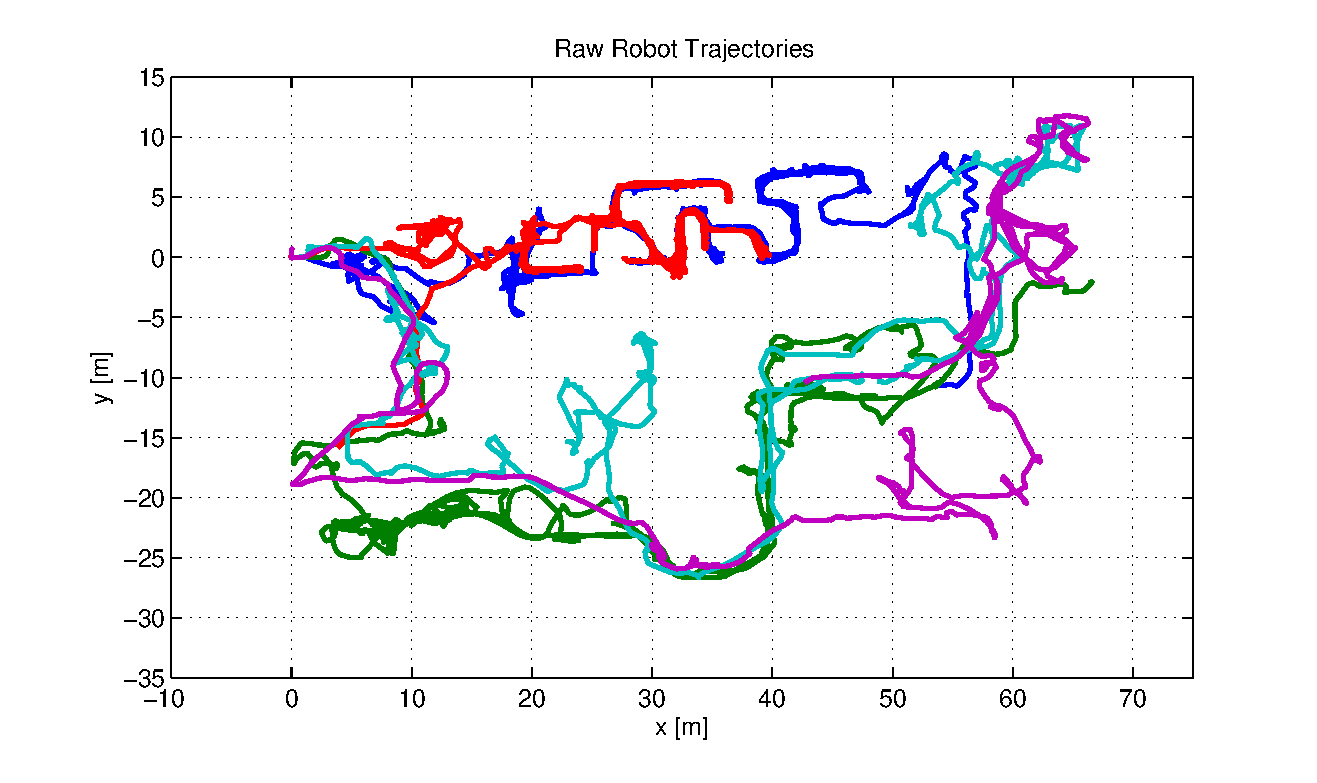
\includegraphics[width=\columnwidth]{fig/raw_traj.pdf}
\caption{Raw trajectory of all robots}
\label{fig:raw_traj}
\end{figure}

%-------------------------------------------------------------------------------
%	PRE-PROCESSING
%-------------------------------------------------------------------------------
\section{Pre-processing}
The data we have is a log file that records raw slam results of 5 robots. Each packet of the data consists of the robot id, the pose of robot at that time, horizontal laser scan in global frame and vertical laser scan in global frame.
In this project, since I'm using scan matching techniques, I didn't use vertical laser data. The preprocessing part is just generate all pose node from the log file. The algorithm is described as follow.
\begin{enumerate}
\item Iterate all possible poses of each robots
\item If a pose is some travel distance away from the previous one, merge all the laser scans around this pose and add to node collection
\item Keep doing this until all poses have been inspected
\item Do 1 to 3 again for another robot
\end{enumerate}
Once we've generated all the nodes in the graph, we can plot all of them with their raw laser scans. We can clearly see from Fig.\ref{fig:raw_node} and \ref{fig:raw_scan} that this raw SLAM result is not perfect and we need to do something to fix it.
\begin{figure}[H]
\centering
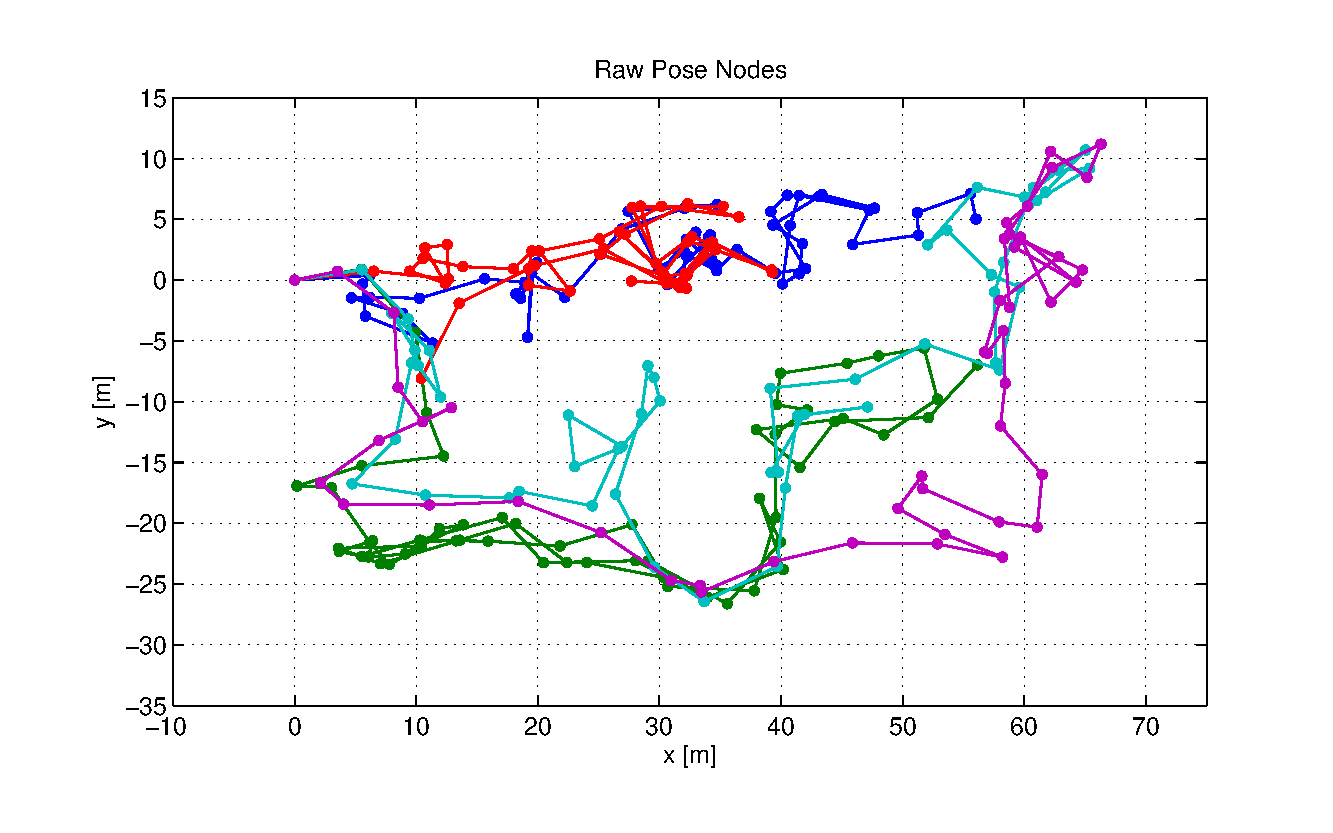
\includegraphics[width=\columnwidth]{fig/raw_node.pdf}
\caption{Raw pose nodes of all robots}
\label{fig:raw_node}
\end{figure}
\begin{figure}[H]
\centering
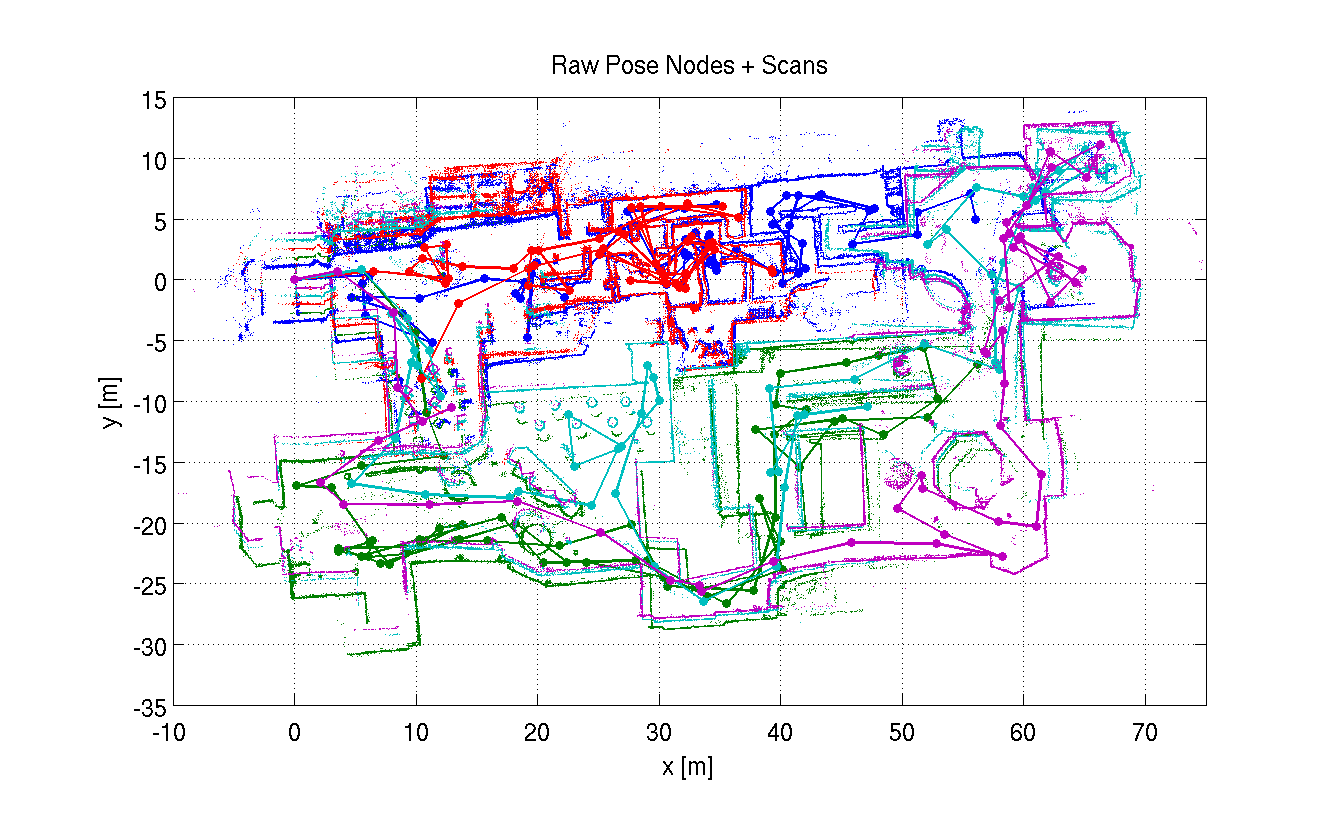
\includegraphics[width=\columnwidth]{fig/raw_scan.pdf}
\caption{Raw pose nodes of all robots with laser scans}
\label{fig:raw_scan}
\end{figure}

%-------------------------------------------------------------------------------
%	METHODS
%-------------------------------------------------------------------------------

\section{Methods}

\subsection{Data Association}
The data association if for finding loop closures. The most popular method for finding 2d laser scan matches is ICP (Iterative Closest Points). Since scan matching is not the main research topic in this project, I simply use a icp library I found online, which is libicp by Andreas Geiger. The result of a loop closure from scan matching is show in \ref{fig:scan_match}.
\begin{figure}[H]
\centering
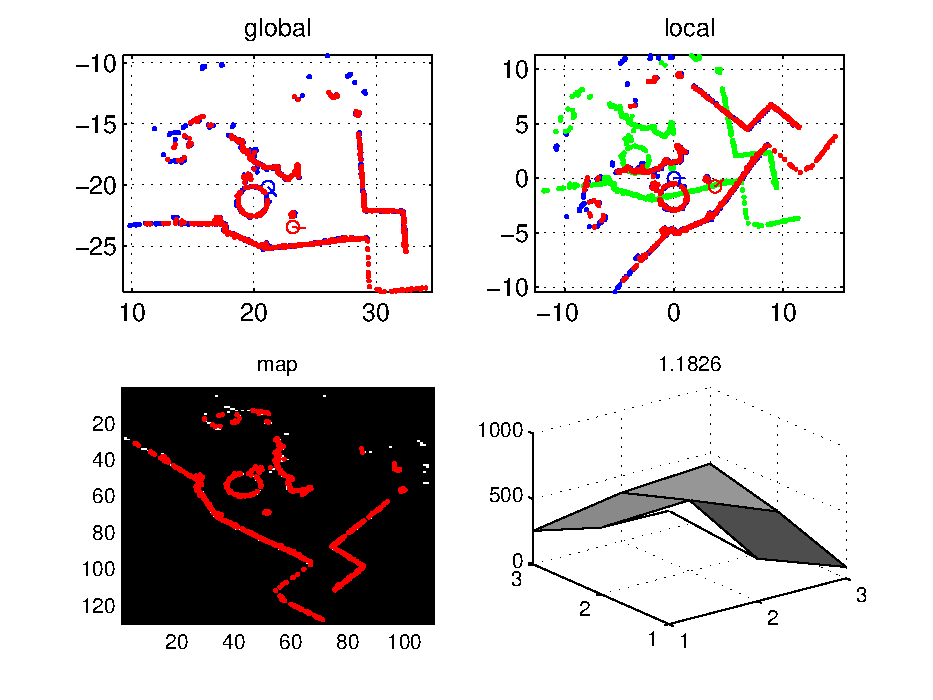
\includegraphics[width=\columnwidth]{fig/scan_match.pdf}
\caption{Scan matching using libicp}
\label{fig:scan_match}
\end{figure}
And the loop closure detection algorithm is also very simple.
\begin{enumerate}
\item Iterate all possible poses of all robots
\item For each pose node, search all the pose nodes before it that satisfy the following results
\begin{enumerate}
\item The node is at least n nodes away from the current node
\item The node is within certain distance of the current node
\end{enumerate}
\item Do scan matching using current node and candidate node
\item If the score returned by scan matcher is higher than some threshold, record both nodes as an edge
\item keep doing this until all nodes have been inspected
\end{enumerate}
The result of data association or loop closure detection is shown in Fig. \ref{fig:loop_closure}. Loop closures are highlighted using black lines.
\begin{figure}[H]
\centering
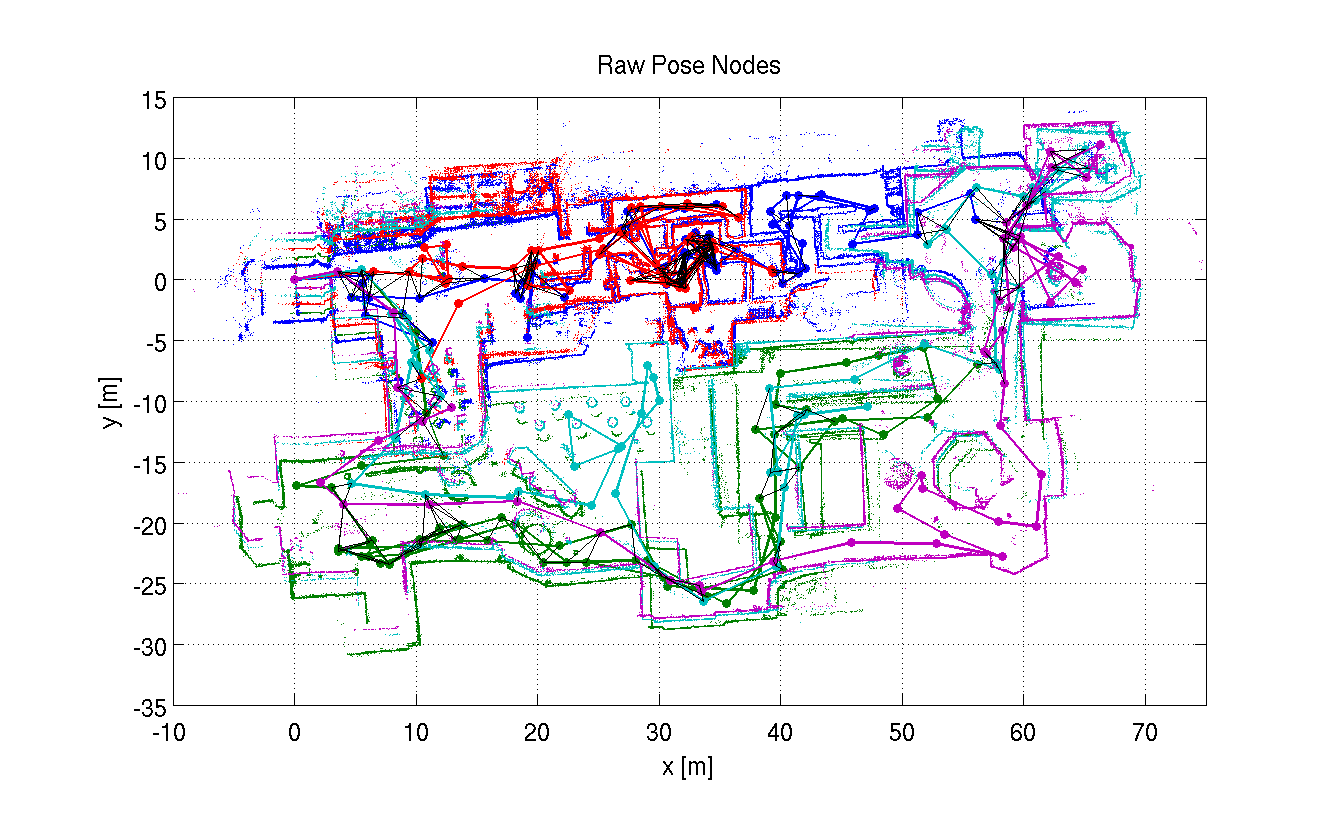
\includegraphics[width=\columnwidth]{fig/loop_closure.pdf}
\caption{Loop closure detection}
\label{fig:loop_closure}
\end{figure}
Assume the inputs to the scan matcher is scans of node i and j in there own local frame. The output is a rototranslation matrix that transform node j's scans into node i's frame. If we convert this rototranslation matrix to a vector form of $\z_{ij} = (x, y, \theta)$, this will be equivalent to a measurement of node j by node i. This result will be used in the following section.\\
Ideally, one would need to calculate covariance or information matrix of each match. To simplify the problem, here we assume fixed covariance.

\subsection{Non-linear Optimization}
The core part of the pose graph SLAM is the non-linear optimization. This part, we closely followed tutorial by Giorgio Grisetti \cite{Giorgio10}. Since the tutorial is very detailed, we will not try to rephrase it, but just highlight some important parts here.
In a pose-graph representation of a SLAM process, every node in the graph corresponds to a robot pose. Poses are connected by edges that model spatial constraints between them. Edges can be modelled by odometry or measurements.
\begin{figure}[H]
\centering
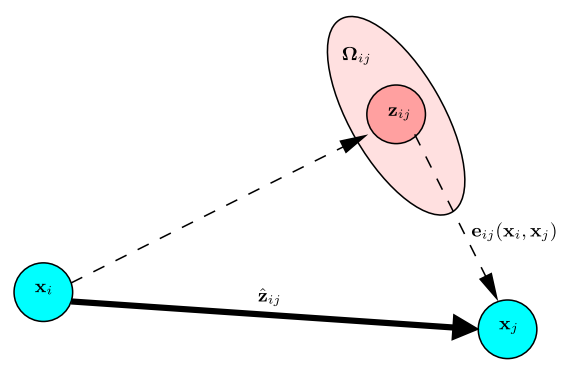
\includegraphics[width=\columnwidth]{fig/virtual_meas.png}
\caption{An edge represented by a virtual measurement}
\label{fig:virtual_meas}
\end{figure}
Let $\x = (\x_1, \ldots, \x_T)^T$ be a vector of robot poses, where $\x_i$ describes the pose of node $i$. Let $\z_{ij}$ and $\omg_{ij}$ be respectively the mean and the information matrix of a virtual measurement between the node $i$ and node $j$. \\
Here a virtual measurement $\z_{ij}$ is simply node $j$ as observed by node $i$, as seen in Fig.\ref{fig:virtual_meas}. The virtual measurement can also be seen as a transformation that makes the observations acquired from $i$ maximally overlap with the observation acquired from $j$. Let $\hat{\z}_{ij}$ is the prediction of a virtual measurement given a configuration of the nodes $\x_i$ and $\x_j$. Usually this prediction is the relative transformation from $\x_j$ to $\x_i$.\\
The likelihood $l_{ij}$ of a measurement is there fore
\begin{equation}
l_{ij} \propto [\z_{ij}-\hat{\z_{ij}}(\x_i,\x_j)]^T\omg_{ij}[\z_{ij}-\hat{\z_{ij}}(\x_i,\x_j)]
\end{equation}
We define $\e(\x_i, \x_j, \z_{ij})$ to be the difference between the predicted observation $\hat{\z_{ij}}$ and the real observation $\z_{ij}$. The objective function we try to minimize is thus
\begin{equation}
\F(\x)=\sum_{\langle i,j \rangle \in \mathcal{C}} \e_{ij}^T \omg_{ij} \e_{ij}
\end{equation}
To which the solution is 
\begin{equation}
\x^* = \mbox{argmin}_\x \F(\x)
\end{equation}
This objective function can be solved by linearizing at a good initial guess $\breve{\x}$ of the robot''s poses. The numerical solution can be obtained by using Gauss-Newton or Levenberg-Marquardt algorithms. We do this by first approximate the error function by its first order Taylor expansion around the current initial guess $\breve{\x}$.
\begin{align}
\F_{ij}&(\breve{\x}+\Delta\x) \\
&= \e_{ij}(\breve{\x}+\Delta	\x)^T \omg_{ij} \e_{ij}(\breve{\x}+\Delta	\x) \\
&= (\e_{ij} + J_{ij}\Delta \x)^T \omg_{ij} (\e_{ij} + J_{ij}\Delta \x) \\
&= \e_{ij}^T \omg_{ij} \e_{ij} + 2\e_{ij}^T \omg_{ij} \J_{ij} \Delta \x + \Delta	\x ^T \J_{ij}\omg_{ij}\J_{ij}\Delta \x \\
&= c_{ij} + 2\mathbf{b}_{ij}\Delta \x + \Delta x^T \mathbf{H}_{ij} \Delta \x
\end{align}
The entire system can be minimized in $\Delta \x$ by solving the linear system
\begin{equation}
\mathbf{H}\Delta \x^* = -\mathbf{b}
\end{equation}
The linearized solution is then obtained b adding to the initial guess the computed increments
\begin{equation}
\x^* = \breve{x}+\Delta \x^*
\end{equation}
This step can be done multiple steps until convergence.
The $\mathbf{H}$ matrix is sparse due to the construction of the graph, thus can be solved efficiently in matlab use sparse matrix inversion.
Fig.\ref{fig:h_matrix} shows the first 300 rows and columns of the $\mathbf{H}$ matrix we generated for this project.
\begin{figure}[H]
\centering
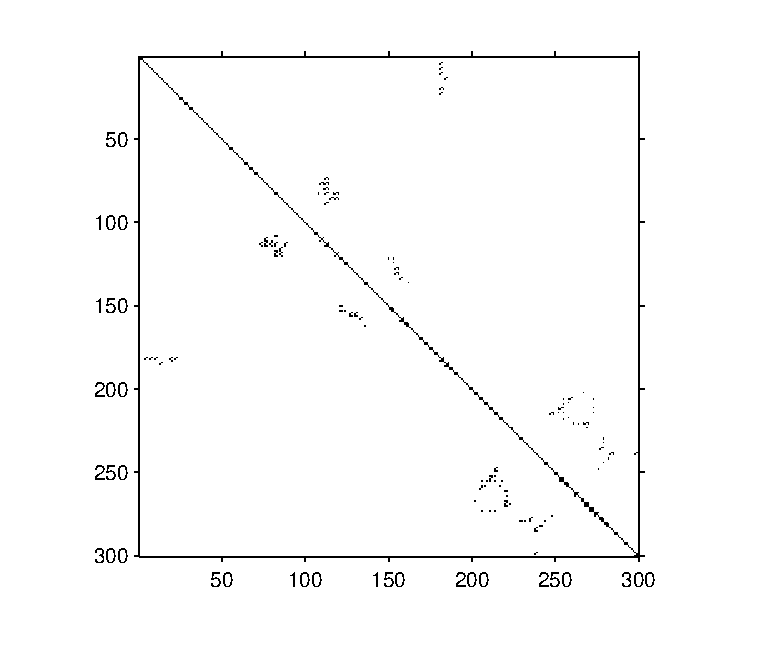
\includegraphics[width=\columnwidth]{fig/h_matrix.pdf}
\caption{A sparse matrix}
\label{fig:h_matrix}
\end{figure}
%-------------------------------------------------------------------------------
%	RESULTS
%-------------------------------------------------------------------------------

\section{Results}
After solving the linear system, we get an improved nodes configuration. 
\begin{figure}[H]
\centering
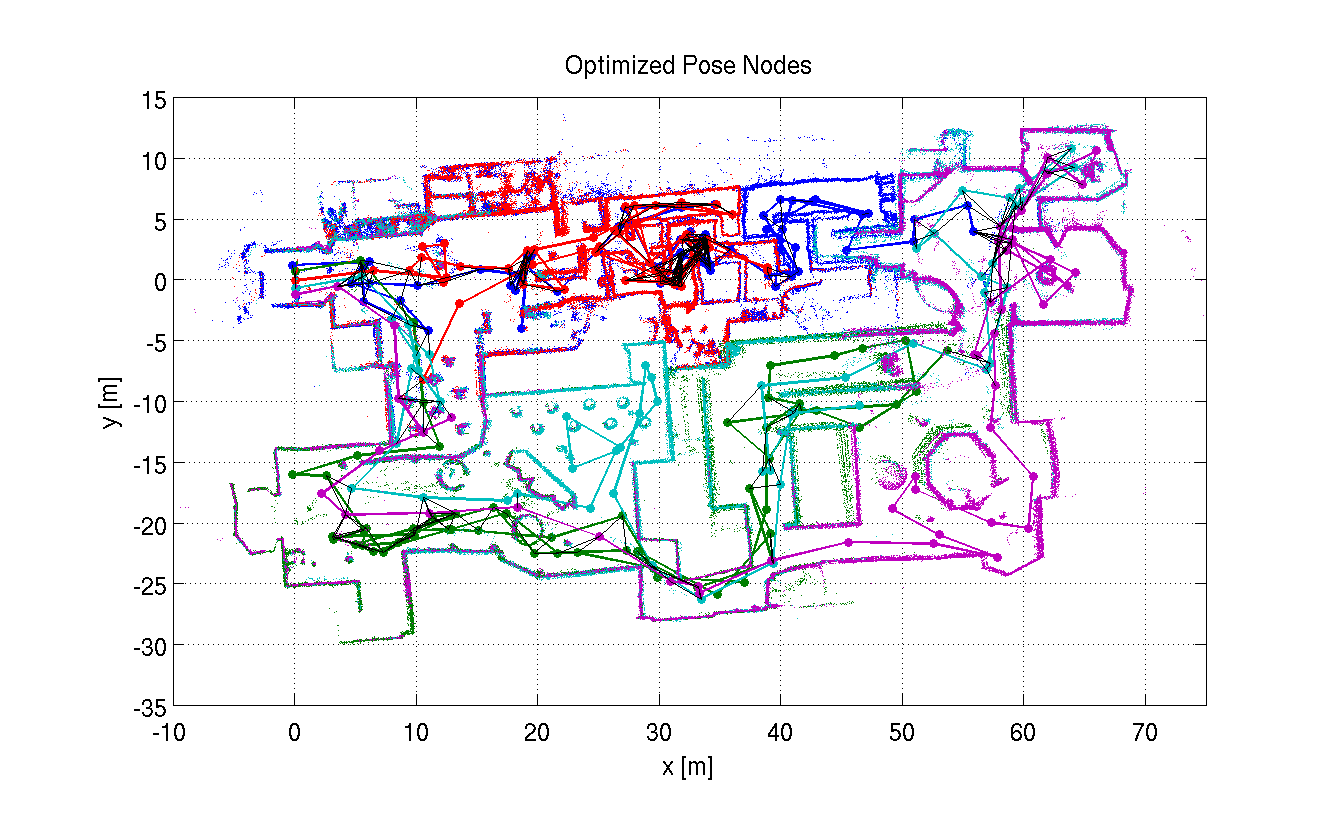
\includegraphics[width=\columnwidth]{fig/opt_scan.pdf}
\caption{Optimized Pose Nodes}
\label{fig:opt_scan}
\end{figure}
We put the raw SLAM plot here for comparison.
\begin{figure}[H]
\centering
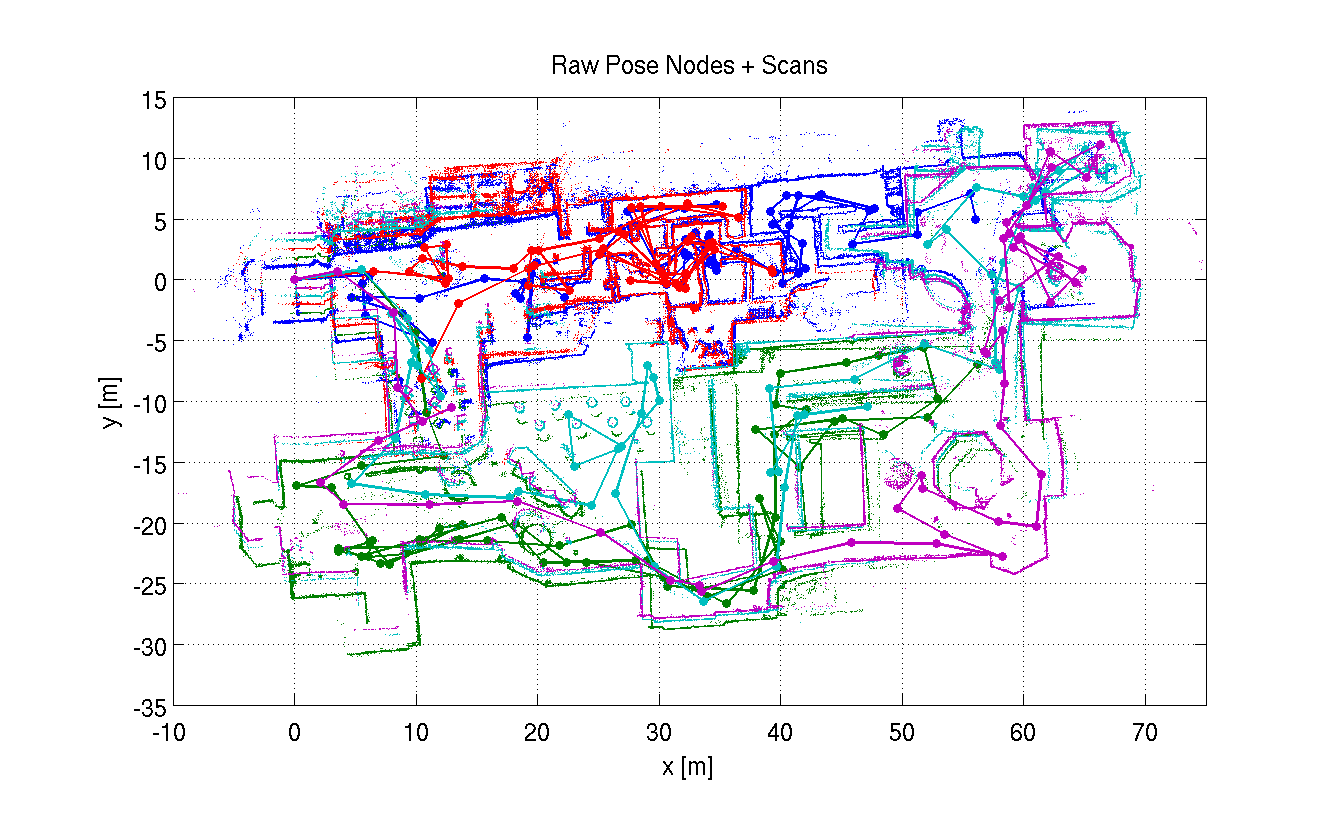
\includegraphics[width=\columnwidth]{fig/raw_scan.pdf}
\caption{Raw Pose Nodes}
\label{fig:raw}
\end{figure}
%-------------------------------------------------------------------------------
%	DISCUSSION
%-------------------------------------------------------------------------------

\section{Discussion}

%-------------------------------------------------------------------------------
%	REFERENCE LIST
%-------------------------------------------------------------------------------

\begin{thebibliography}{2} % Bibliography - this is intentionally simple in this template

\bibitem{Giorgio10}
G.Grisetti, R. Kummerle, C. Stachniss et al., \emph{A Tutorial on Graph-Based SLAM}. Intelligent Transportation Systems Magazine, IEEE (Volume:2, Issue:4), 2000.
%
%\bibitem{Elmez07}
%Elmezain M. and Al-Hamadi A., \emph{A Hidden Markov Model-based continuous gesture recognition system for hand motion trajectory}. 19th International Conference on Pattern Recognition, ICPR 2008.
%
%\bibitem{Rabiner89}
%Lawrence R. Rabiner, \emph{A Tutorial on Hidden Markov Models and Selected Applications in Speech Recognition}. Proceedings of the IEEE, 1989.

\end{thebibliography}

%-------------------------------------------------------------------------------

\end{multicols}

\end{document}
